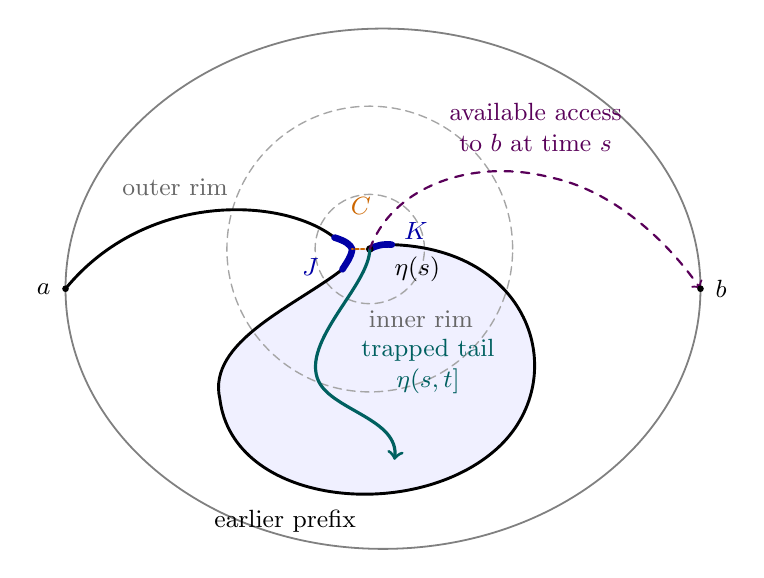
\begin{tikzpicture}[x=1.12cm,y=1.12cm,
    line cap=round,line join=round,font=\small,
    gateprefix/.style={black,line width=1.05pt},
    piece/.style={blue!65!black,line width=2.4pt},
    gate/.style={orange!80!black,line width=1.05pt,densely dotted},
    future/.style={teal!75!black,line width=1.15pt,->},
    access/.style={violet!70!black,line width=.8pt,dashed,->},
    rim/.style={black!35,line width=.5pt,dash pattern=on 3pt off 2pt}]
  \coordinate (a) at (-3.6,0);
  \coordinate (b) at (3.6,0);
  \coordinate (j) at (-.35,.45);
  \coordinate (s) at (-.15,.45);

  \path[fill=blue!6]
    (j) .. controls (-.36,.36) and (-.41,.30) .. (-.46,.22)
    .. controls (-1,-.20) and (-2,-.60) .. (-1.85,-1.25)
    .. controls (-1.70,-2.45) and (.30,-2.65) .. (1.25,-1.85)
    .. controls (2.15,-1.10) and (1.75,.45) .. (.10,.50)
    .. controls (0,.51) and (-.08,.49) .. (s)
    -- (j) -- cycle;

  \draw[black!50,line width=.65pt] (0,0) ellipse (3.6 and 2.95);
  \draw[rim] (s) circle (.62);
  \draw[rim] (s) circle (1.62);
  \node[black!60] at (.43,-.34) {inner rim};
  \node[black!60,anchor=east] at (-1.65,1.15) {outer rim};

  \draw[gateprefix]
    (a) .. controls (-2.70,1.10) and (-1.15,1.05) .. (-.55,.58)
    .. controls (-.42,.54) and (-.37,.50) .. (j)
    .. controls (-.36,.36) and (-.41,.30) .. (-.46,.22)
    .. controls (-1,-.20) and (-2,-.60) .. (-1.85,-1.25)
    .. controls (-1.70,-2.45) and (.30,-2.65) .. (1.25,-1.85)
    .. controls (2.15,-1.10) and (1.75,.45) .. (.10,.50)
    .. controls (0,.51) and (-.08,.49) .. (s);

  \draw[piece]
    (-.55,.58) .. controls (-.42,.54) and (-.37,.50) .. (j)
    .. controls (-.36,.36) and (-.41,.30) .. (-.46,.22);
  \draw[piece]
    (.10,.50) .. controls (0,.51) and (-.08,.49) .. (s);
  \node[blue!65!black,anchor=east] at (-.62,.25) {$J$};
  \node[blue!65!black,anchor=west] at (.13,.65) {$K$};

  \draw[gate] (s) -- (j);
  \node[orange!80!black,anchor=south] at (-.25,.73) {$C$};
  \fill (s) circle (1.35pt);
  \node[anchor=west] at (.02,.22) {$\eta(s)$};

  \draw[future]
    (s) .. controls (-.15,.04) and (-.94,-.60) .. (-.73,-1.05)
    .. controls (-.57,-1.38) and (.19,-1.48) .. (.13,-1.94);
  \node[teal!75!black,align=center] at (.51,-.88)
    {trapped tail\\$\eta(s,t]$};

  \draw[access]
    (s) .. controls (.11,1.17) and (1.03,1.49) .. (1.91,1.26)
    .. controls (2.57,1.12) and (3.18,.60) .. (b);
  \node[violet!70!black,align=center] at (1.73,1.83)
    {available access\\to $b$ at time $s$};

  \fill (a) circle (1.2pt);
  \fill (b) circle (1.2pt);
  \node[anchor=east] at (-3.66,0) {$a$};
  \node[anchor=west] at (3.66,0) {$b$};
  \node[anchor=north] at (-1.11,-2.40) {earlier prefix};
\end{tikzpicture}

